\documentclass[a4paper,11pt]{article}
\usepackage[english]{babel} 
\usepackage[hmargin=2cm,vmargin=2.5cm]{geometry} 

\usepackage{caption}
\usepackage{subcaption} 
\usepackage{float}

\usepackage{graphics}
\usepackage{graphicx}

\usepackage{comment} 
\usepackage{paralist}

\usepackage{amssymb}
\usepackage{amsmath}
\usepackage{amsfonts}

\graphicspath{{.}{images/}}
\newcommand{\degree}{\ensuremath{^\circ}}

\usepackage{hyperref}

\usepackage[nonumberlist]{glossaries}
%\newcommand{\dictentry}[2]{\begin{quotation}\textbf{#1}: #2\end{quotation}}
\newcommand{\dictentry}[2]{%
  \newglossaryentry{#1}{name=#1,description={#2}}%
}
\makeglossaries

\begin{document}

\begin{center}
{\LARGE \textsc{Alignment in asymmetric interactions \\ First thoughts and results} \\ [0.2cm]
{\large \textbf{Last update:} \today}} \\ [0.2cm]
\end{center}

\begin{abstract}
This document is meant to summarize the current ideas and initial results from the human experiments we performed this summer. Those experiments were initially designed to study communication between humans in situation similar to simple human-robot interaction scenario.
\end{abstract}

%comment unwanted section
\dictentry{Frames}{Social behavioural pattern that guide social interaction by providing predictable, recurrent interactive structures. Embedding a new word within a familiar frame results in the reduction of the information load as this word will be perceived as a new slot within a familiar routine}

\dictentry{Pragmatics}{Subfield of linguistics which studies the ways in which context contributes to meaning. Pragmatics studies how the transmission of meaning depends not only on structural and linguistic knowledge (e.g., grammar, lexicon, etc.) of the speaker and listener, but also on the context of the utterance, any pre-existing knowledge about those involved, the inferred intent of the speaker, and other factors. In this respect, pragmatics explains how language users are able to overcome apparent ambiguity, since meaning relies on the manner, place, time etc.\ of an utterance}

\dictentry{Theory of mind}{Ability to attribute mental states --- beliefs, intents, desires, pretending, knowledge, etc. --- to oneself and others and to understand that others have beliefs, desires, and intentions that are different from one's own. Deficits occur in people with autism spectrum disorders, schizophrenia, attention deficit hyperactivity disorder, as well as neurotoxicity due to alcohol abuse}

\dictentry{Confirmation bias}{Tendency of people to favour information that confirms their beliefs or hypotheses. People display this bias when they gather or remember information selectively, or when they interpret it in a biased way. The effect is stronger for emotionally charged issues and for deeply entrenched beliefs. They also tend to interpret ambiguous evidence as supporting their existing position. Biased search, interpretation and memory have been invoked to explain attitude polarization (when a disagreement becomes more extreme even though the different parties are exposed to the same evidence), belief perseverance (when beliefs persist after the evidence for them is shown to be false), the irrational primacy effect (a greater reliance on information encountered early in a series) and illusory correlation (when people falsely perceive an association between two events or situations)}



\section{Thoughts}

This section summarize few thoughts developed during meetings, mail exchanges and reading of the pragmatic frames paper \cite{rohlfing2013learning}. A small glossary is available at the end of the document.

It is important to note that, in our human experiment and algorithm framework, we are not focused on how to acquired new abilities but rather on how two agents can understand each other in asymmetric interaction. We assume that there is a pre-defined interaction goal or context (building something with blocks) and that both participant knowns how to complete a task inside this context. In our algorithmic framework we assume there is a shared knowledge on the pragmatic frame used in the interaction. While in the human experiment, even if no frames are explicitly given, participants are adults and are already familiar with a multitude of possible frames to apply in such situation. In this case participants needs to agree on which frame(s) their interaction is based on, and which buttons are used to mean what inside this frame.

I would like to explicitly details this point as I think the vocabulary we are learning from this community is very relevant for us. In our human experiment, we could argue that both side are trying to ground the interaction into known frames of interaction. When trying to infer the current mental state of the other, people tend to look for pattern similar to known, and ``universally shared'', interaction frames. Indeed, adults have already acquired complex pragmatics frames which may include feedback, guidance, location or colour naming. The use of the pragmatics is used to identify which signal means what in the context of a frame.
\begin{itemize}
    \item The student uses its knowledge about the possible tasks to ground the signal appearing on the screen to some meaning into a frame. Frame that they believe the teacher may be using with regard to the current state of the interaction.
    \item The teacher uses its observation of the student behaviour to select a particular frame (and press the button accordingly).
\end{itemize}
Some specific signals can also be identified as conveying a certain state of mind. But their interpretation will depend on the current state of the interaction. As an example: a highly unexpected signals, e.g.\ all buttons pressed, may be commonly accepted as a ``stop and pay attention'' signal which according to the context, i.e.\ if the student feel confident or not, may be interpreted as a ``reset'' or a ``finish''.
\\

The first conclusion that as been derived by Katharina is that those experiments are more related to alignment (for more info about alignment see \cite{pickering2004toward}). However, to her knowledge, alignment was not studied in teaching scenarios, i.e.\ in asymmetric interactions, which makes our experiment innovative.

A second perspective is to use this setup for different types of task (construction, classification, \ldots) and study what types of instructions are emerging on each cases. What are the conditions, the basics, of each type of instruction signal. 

A third immediate perspective is on the algorithm side. We could also embed a set of frames inside our robot/agent and try to match to ongoing interaction to one of such frames. That would make hypothesis on both side, tasks and frames. 
\\

We may sometime have some vocabulary misunderstandings due to our respective fields.  The main one is probably on the term ``feedback'' which we tend to use for the specific positive and negative assessment of action while, I think, Katharina is using in a more general term, as an indication from a teacher to a learner.

Additionally, perhaps the word \emph{teacher} and \emph{student} are not adapted to this scenario. It is more like an \emph{architect} and a \emph{worker}, they both know how to build a tower but the architect should explain which tower he wants to be build.
\\

Finally, on an other perspective, I think Katharina would be really interested in building system that can learn (and later use) frames.

\section{Experiments}

Based on \cite{griffiths2012bottom}, we wanted to remove the learner's access to a performance measure so as to create an interaction similar to what we have in \cite{grizou2013robot}.

\subsection{Method}

%In this experiment, we investigate how adult can negotiate

The purpose of this experiment was to simulate a basic human-robot interaction and study how human adults would perform in such situation. Specifically, the learner does not have access to a measure of its performance; the teacher can only understand the intention of the learner thought its external, not explicitly communicative, behaviour; and the learner can only process information in a sequence of symbolic signals. To illustrate this scenario, we consider a construction task, were a teacher must explain to a learner what construction must be build with the blocks present on a table.


\subsubsection{Participants}

The 36 participants (31 M / 5 F), recruited among students and staff at INRIA Bordeaux Sud-Ouest, were divided into teachers and learners. They registered to be participants beforehand. The age range was between 20 and 35 and their average was 24 years.

\subsubsection{Stimuli}

The teacher and the student were in separate rooms and had only access to selected information displayed on a screen. For the purpose of the present study, we developed a simple computer interface. On the student side, a computer was displaying symbols associated to button-presses from the teacher. On the teacher side, a computer was displaying the blocks moved by the student recorded by a webcam on the student side. To send signals to the student the teacher had access to a box equipped with 10 buttons, see figure~\ref{fig:box}. Each button was randomly mapped to a symbols and screen position on the student side. We tried to use neutral symbols, see figure~\ref{fig:sign}.

There were 12 primary-coloured Mega Blocks$^{\textregistered}$ blocks of different size (see figure~\ref{fig:duplos}); 3 red two-pads, 2 red three-pads, 2 yellow four-pads, 2 blue three-pads, 2 green two-pads, and 1 green four-pads blocks. During preliminary tests, we found that leaving the teacher with a free choice for the aimed construction was unproductive. We therefore presented the teacher with 20 construction's pictures from which they should choose one, see figure~\ref{fig:constructions}. A construction does not necessary contain every blocks.

\begin{figure}[H]	
	\centering
	\begin{subfigure}[t]{0.32\columnwidth}
		\centering
		
\includegraphics[width=\columnwidth]{sign.png}
		\caption{Three examples of sign displayed on the learner screen}\label{fig:sign}		
	\end{subfigure}
	\begin{subfigure}[t]{0.32\columnwidth}
		\centering
		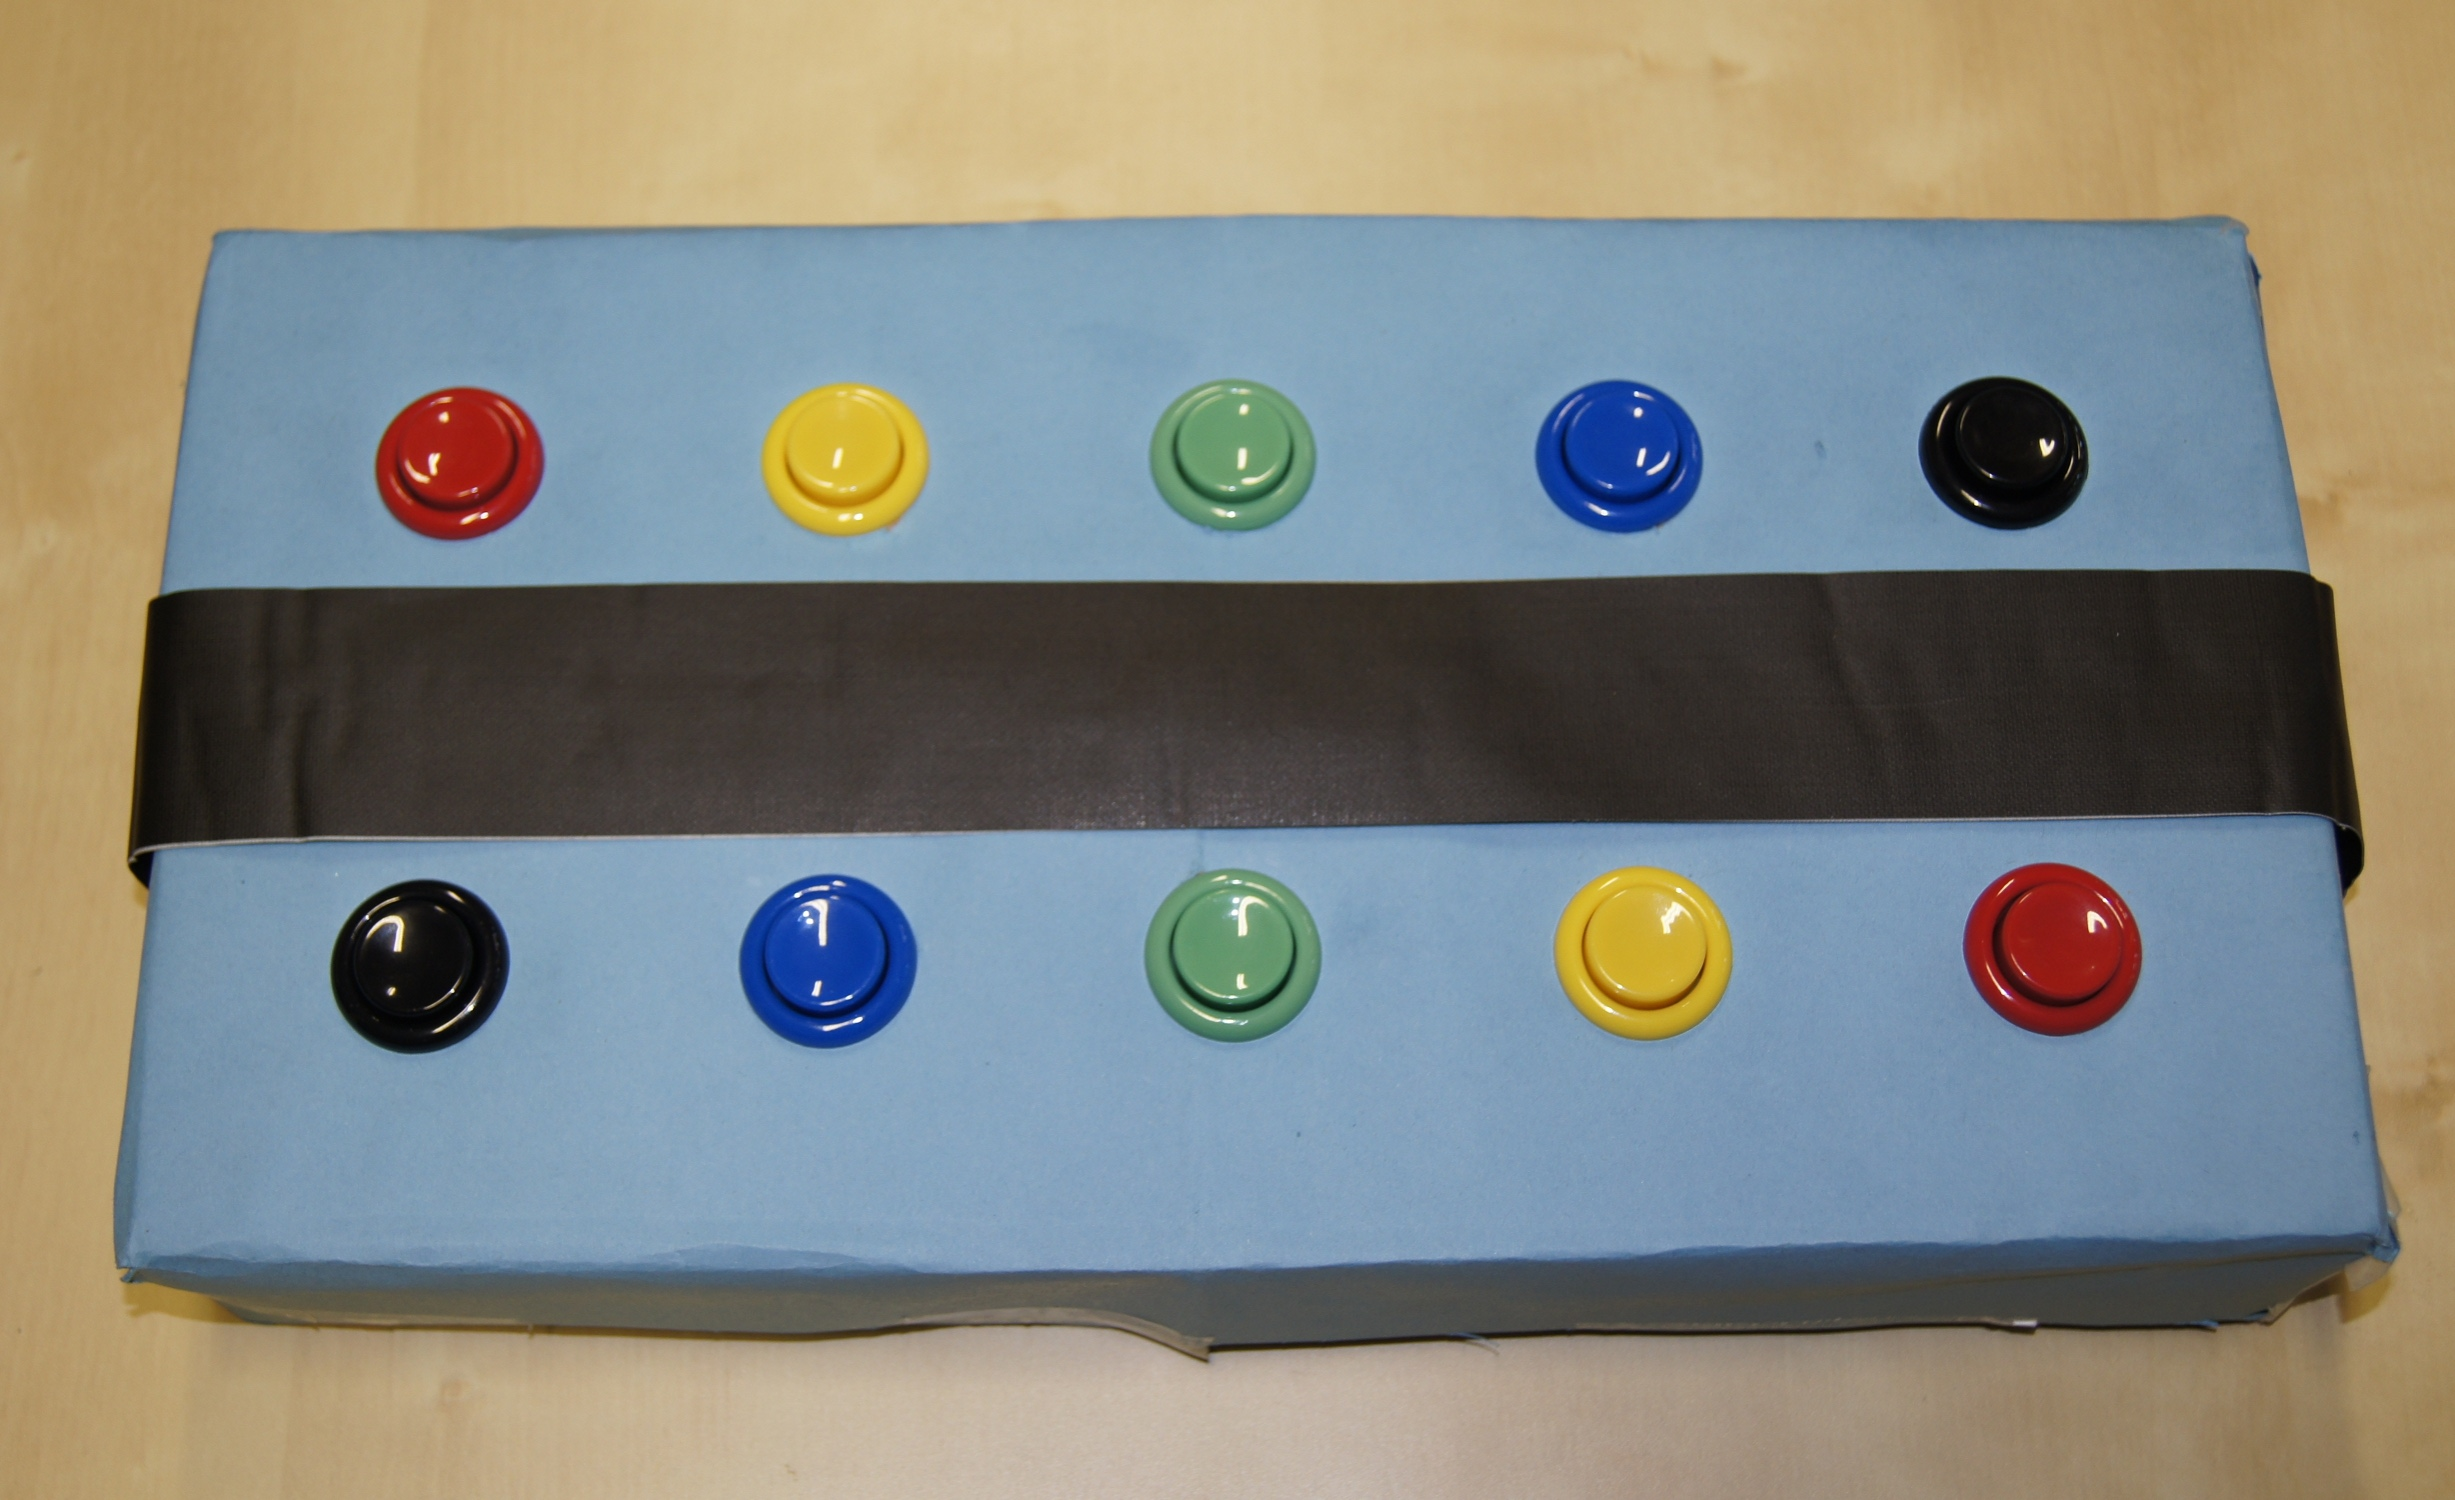
\includegraphics[width=\columnwidth]{box.jpg}
		\caption{The box and the button use as an interface for the teacher to communicate with the learner}\label{fig:box}
	\end{subfigure}
	\begin{subfigure}[t]{0.32\columnwidth}
		\centering
		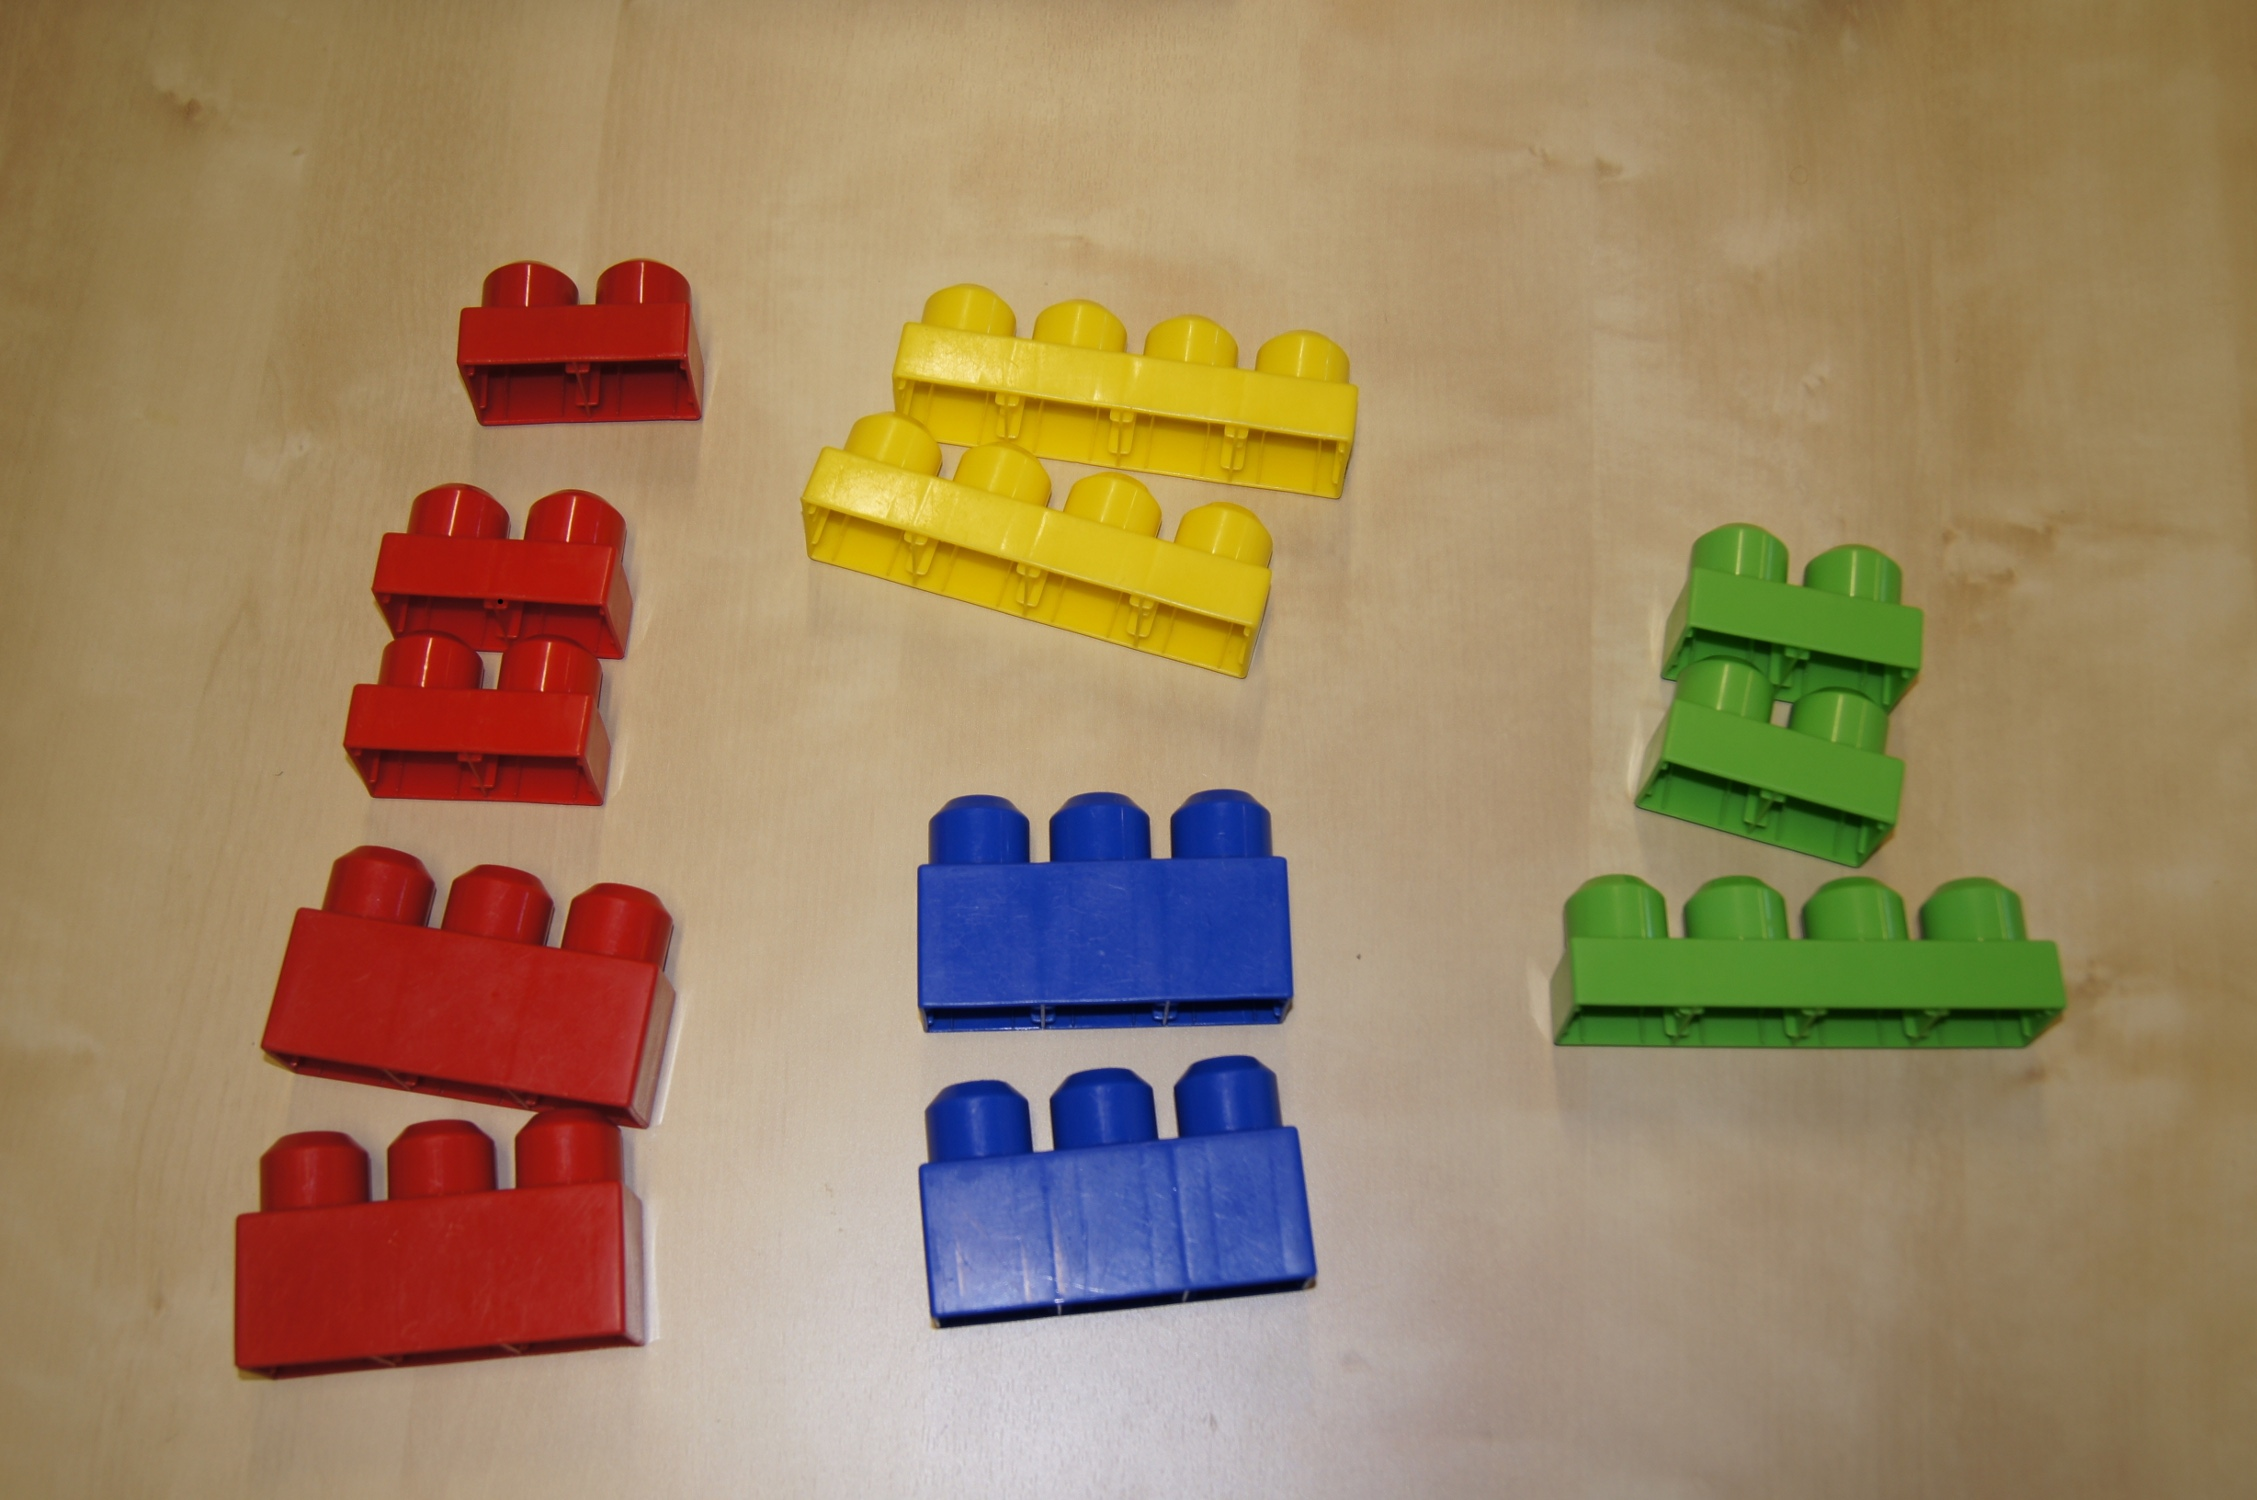
\includegraphics[width=\columnwidth]{duplos.jpg}
		\caption{The blocks used in the construction task}\label{fig:duplos}
	\end{subfigure}
	\begin{subfigure}[b]{\columnwidth}
		\centering
		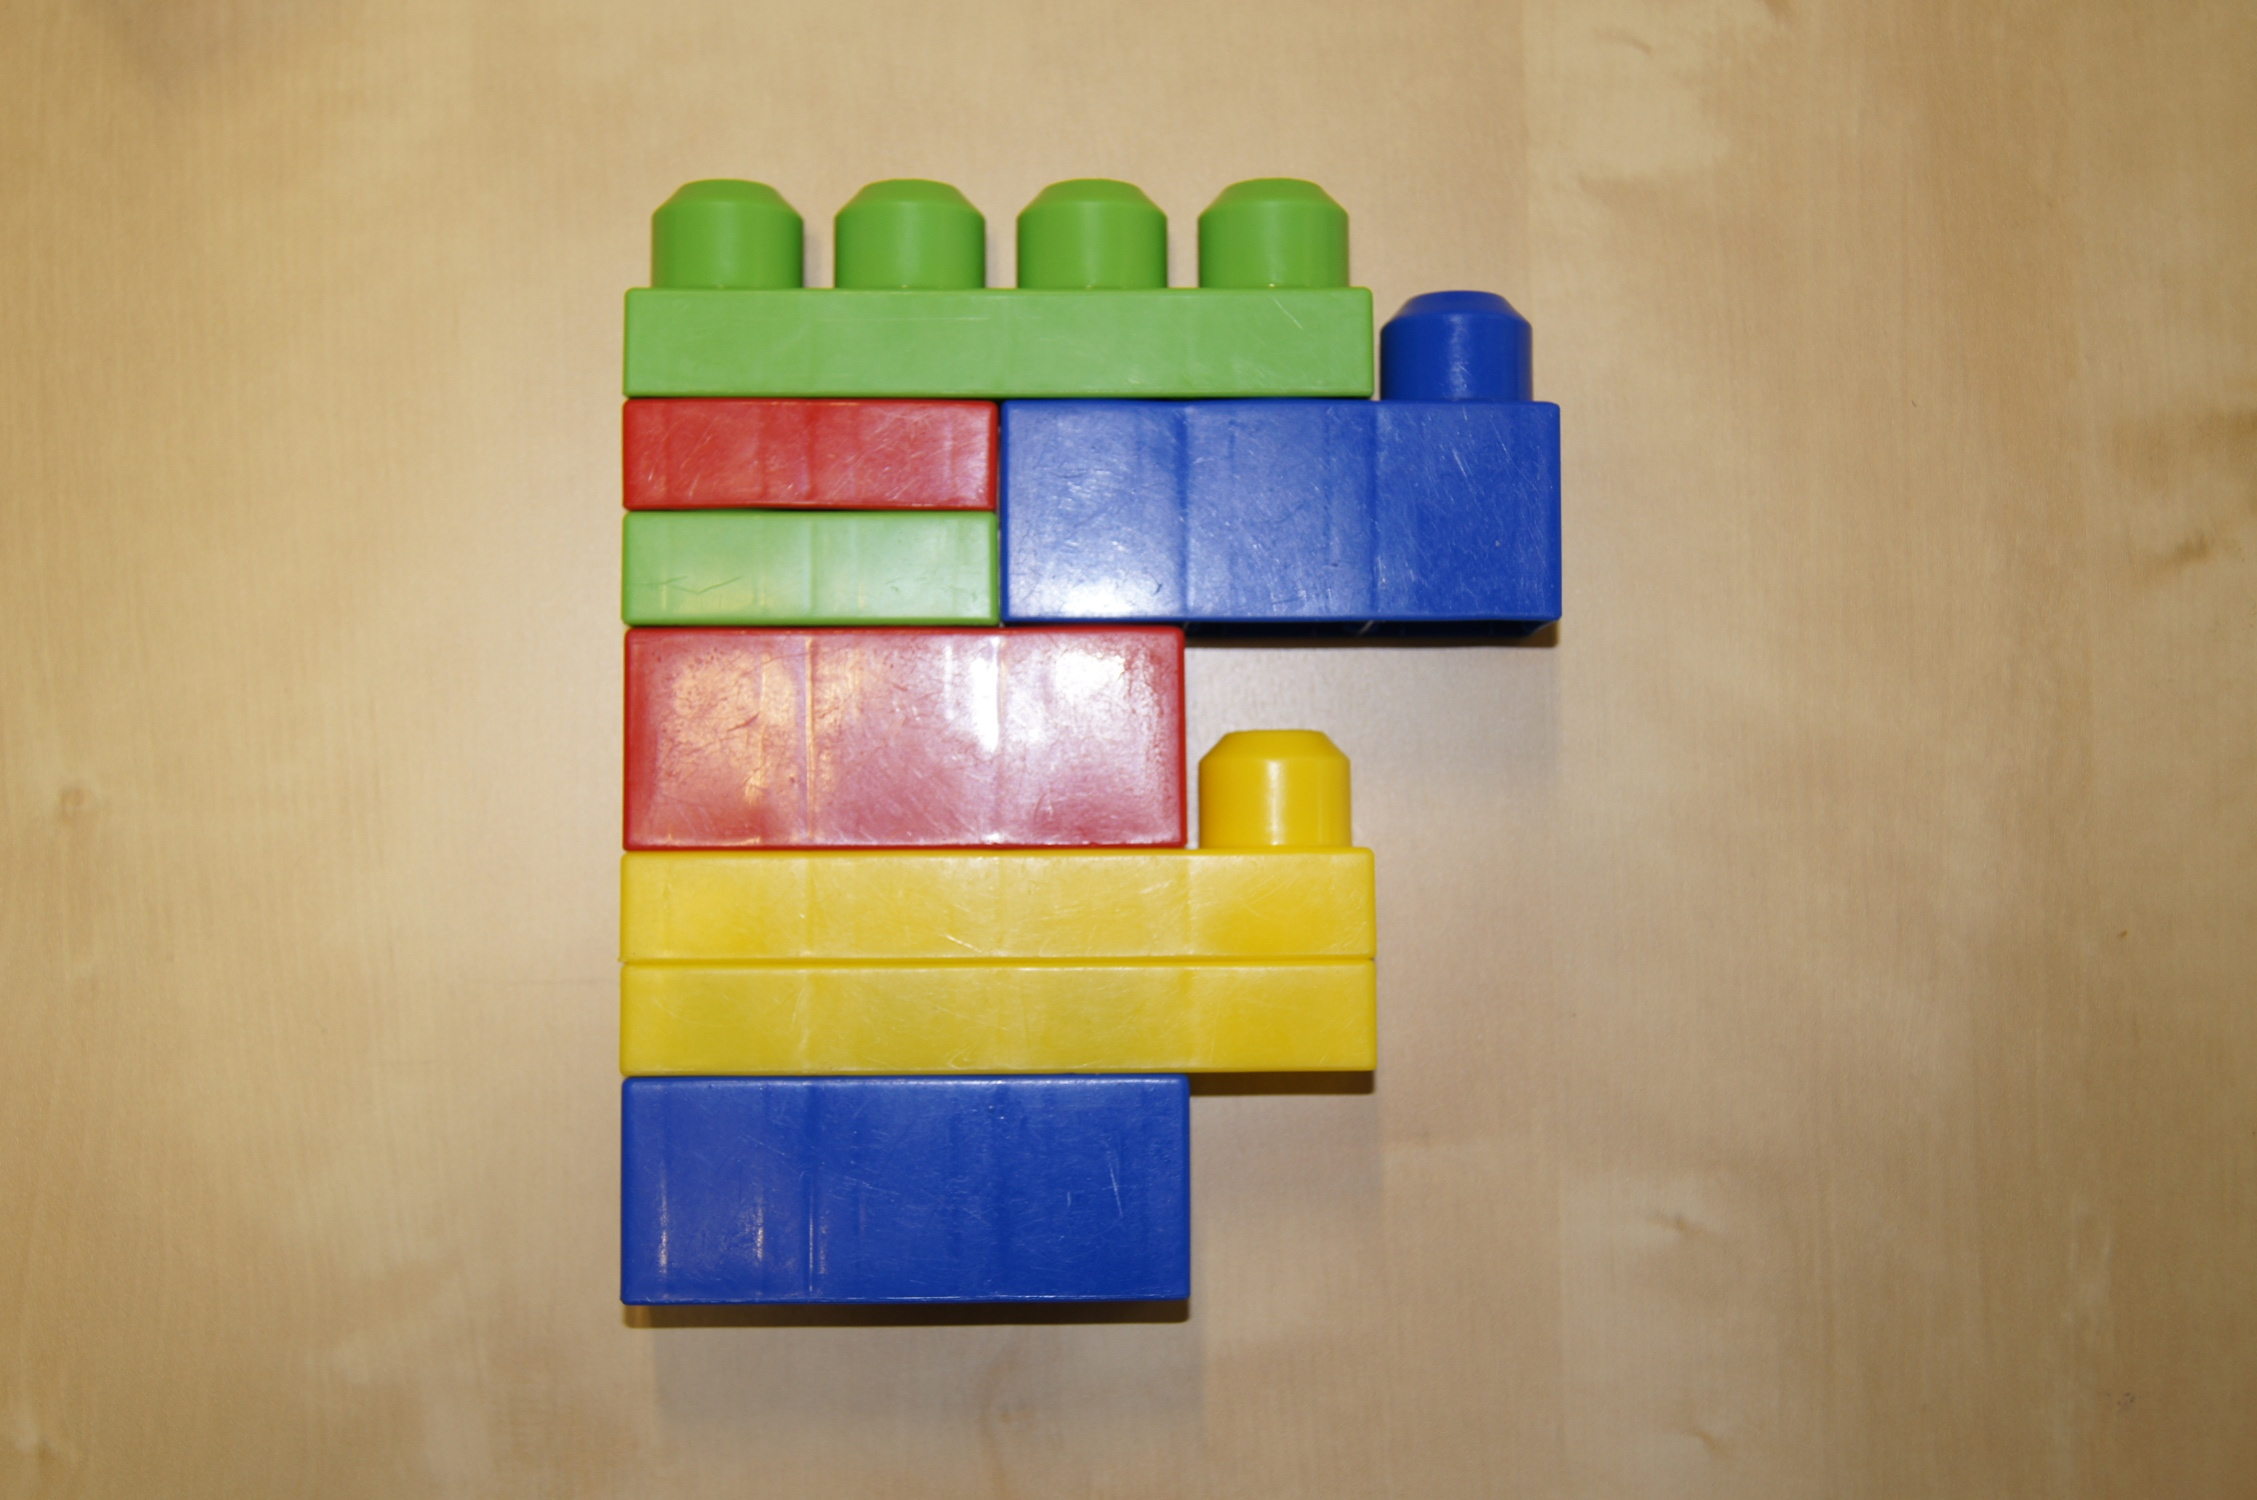
\includegraphics[width=0.24\columnwidth]{foo/_DSC4111.JPG}
		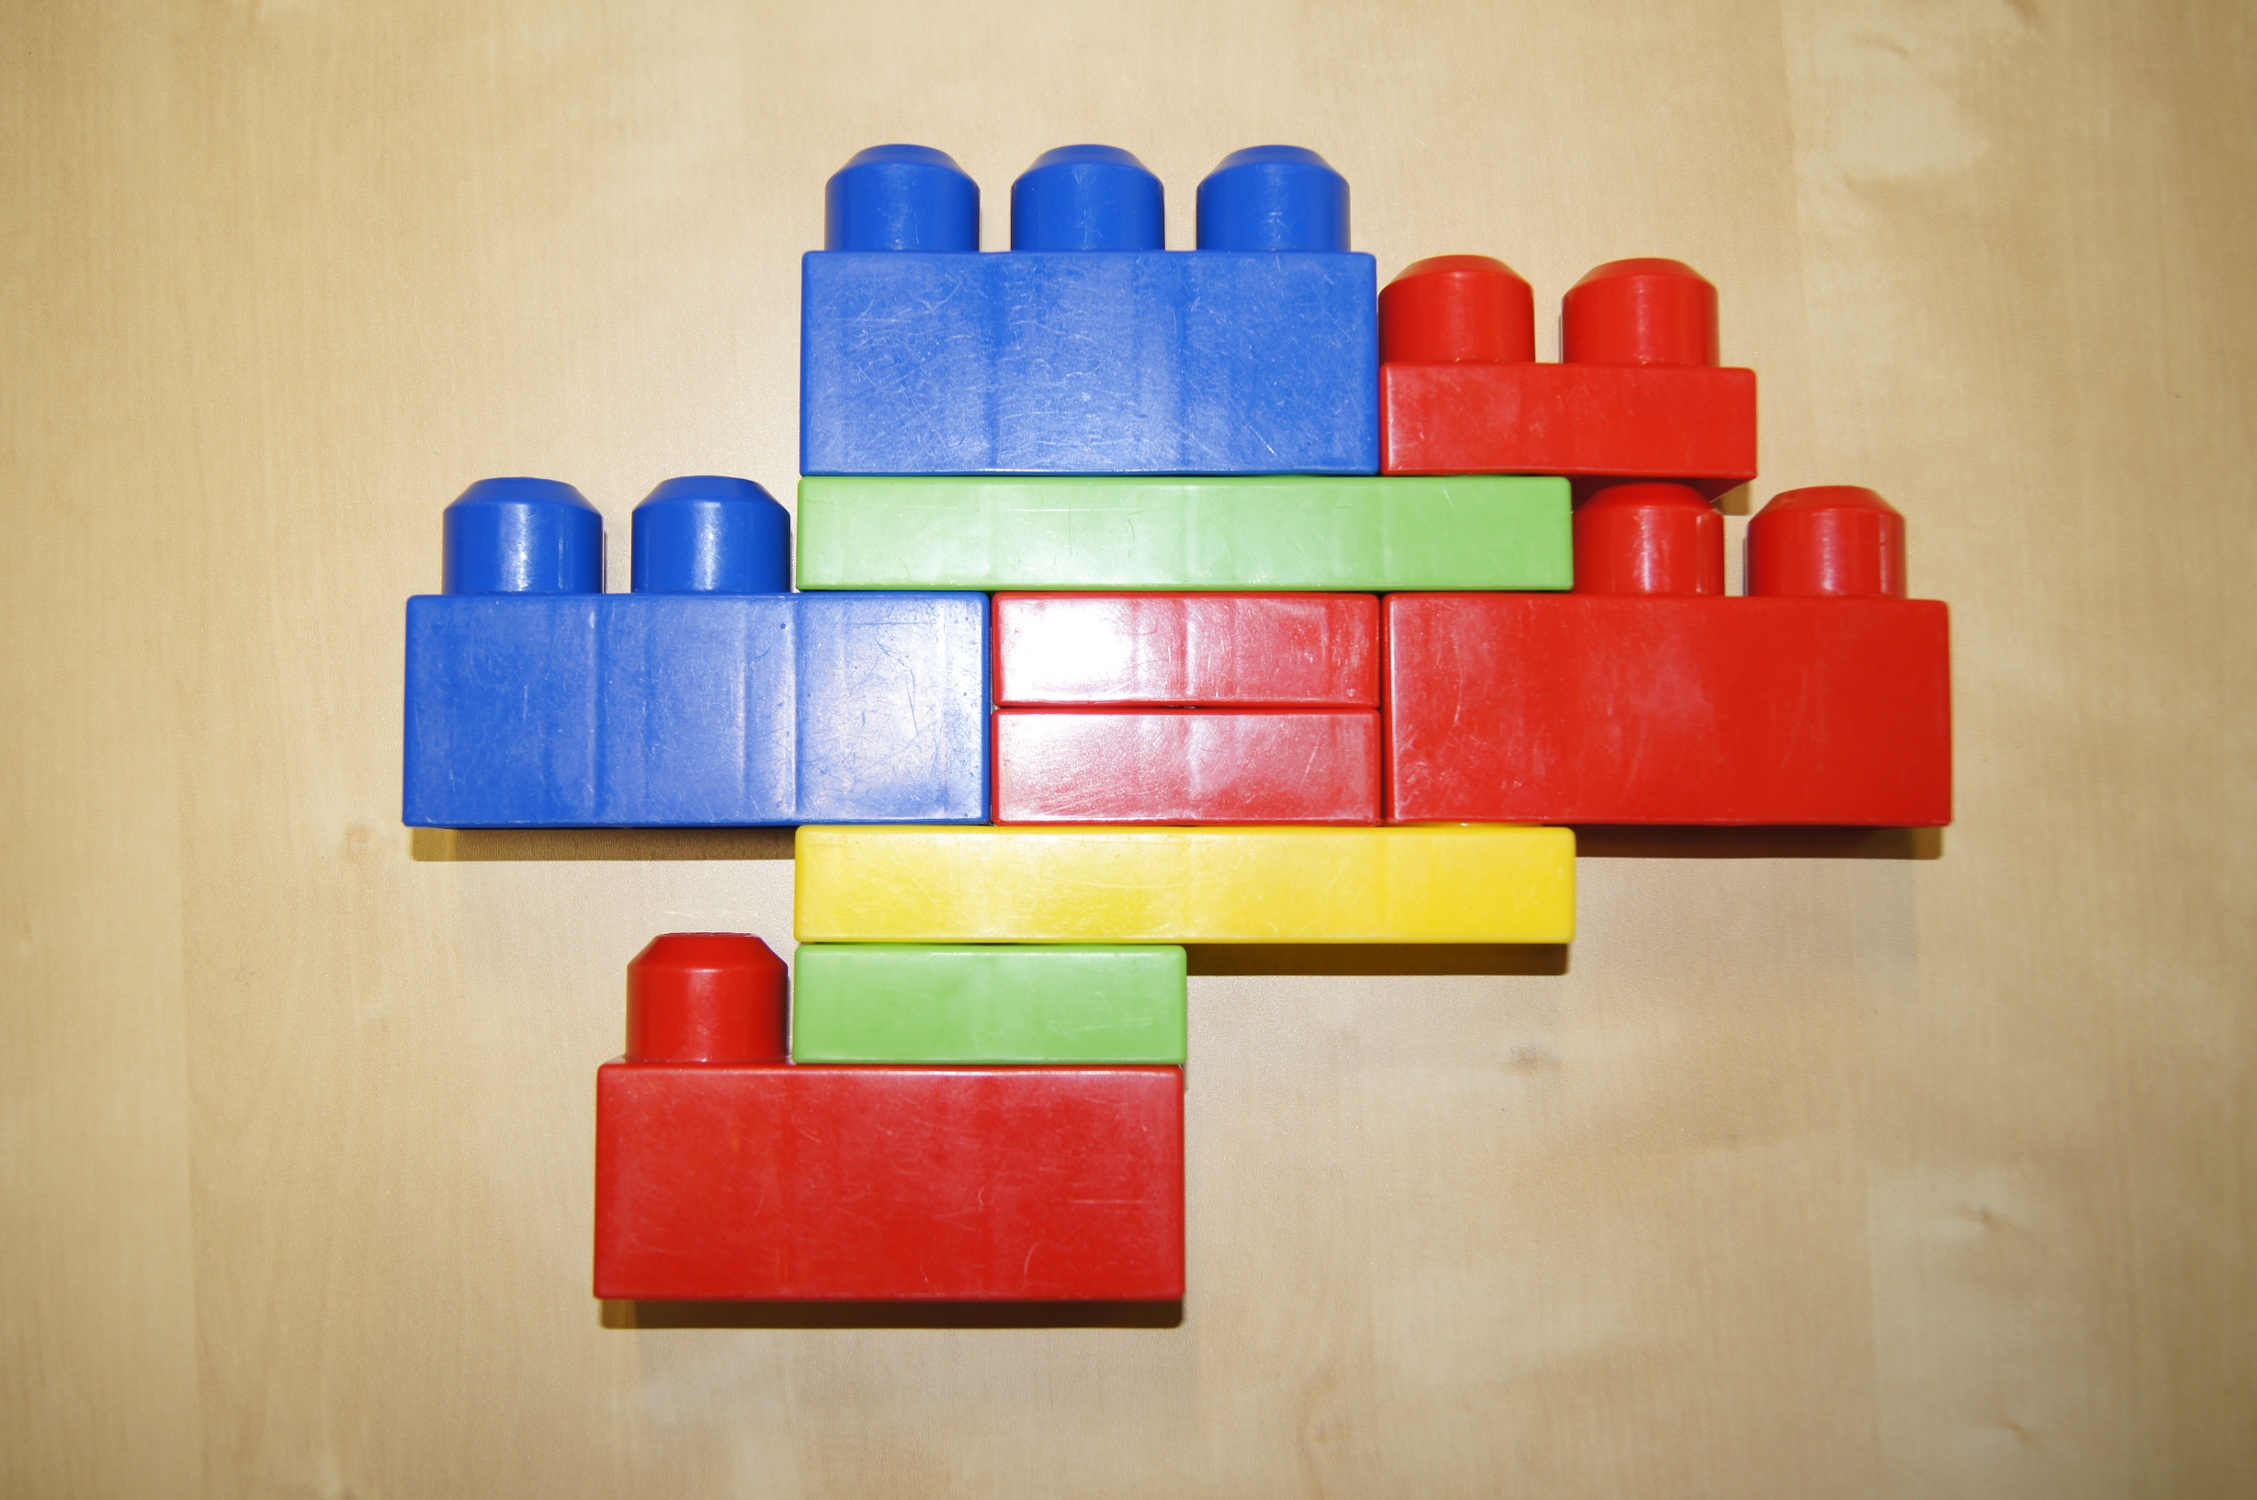
\includegraphics[width=0.24\columnwidth]{foo/_DSC4119.JPG}
		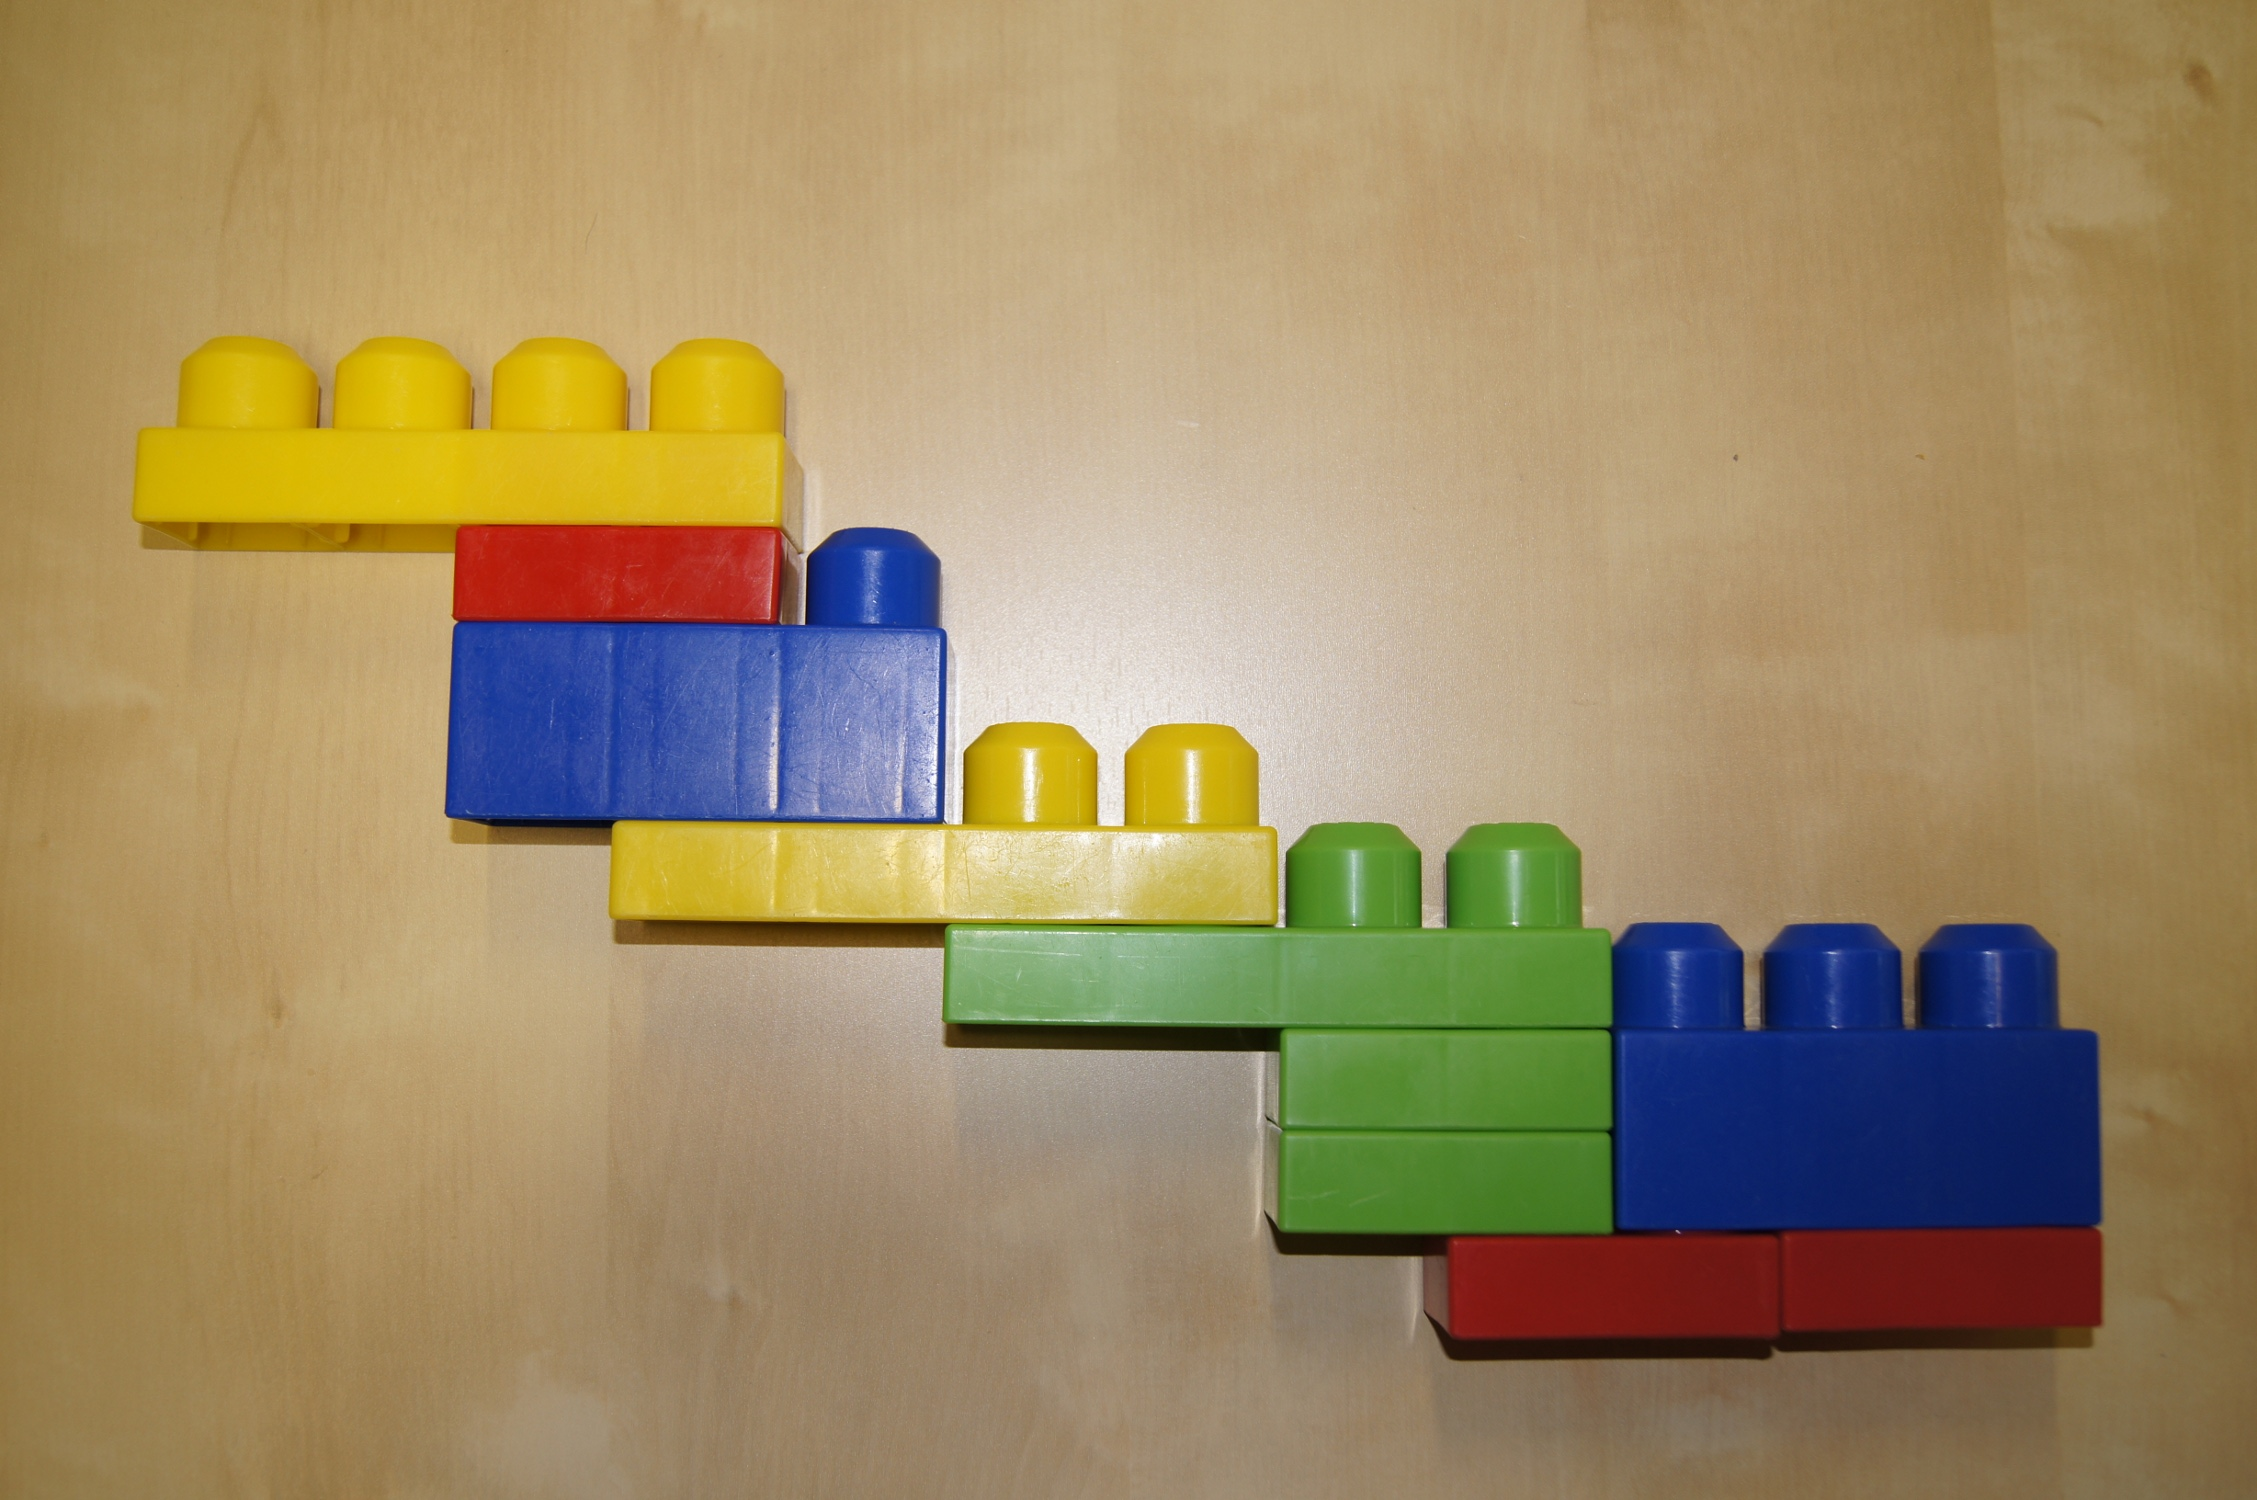
\includegraphics[width=0.24\columnwidth]{foo/_DSC4115.JPG}
		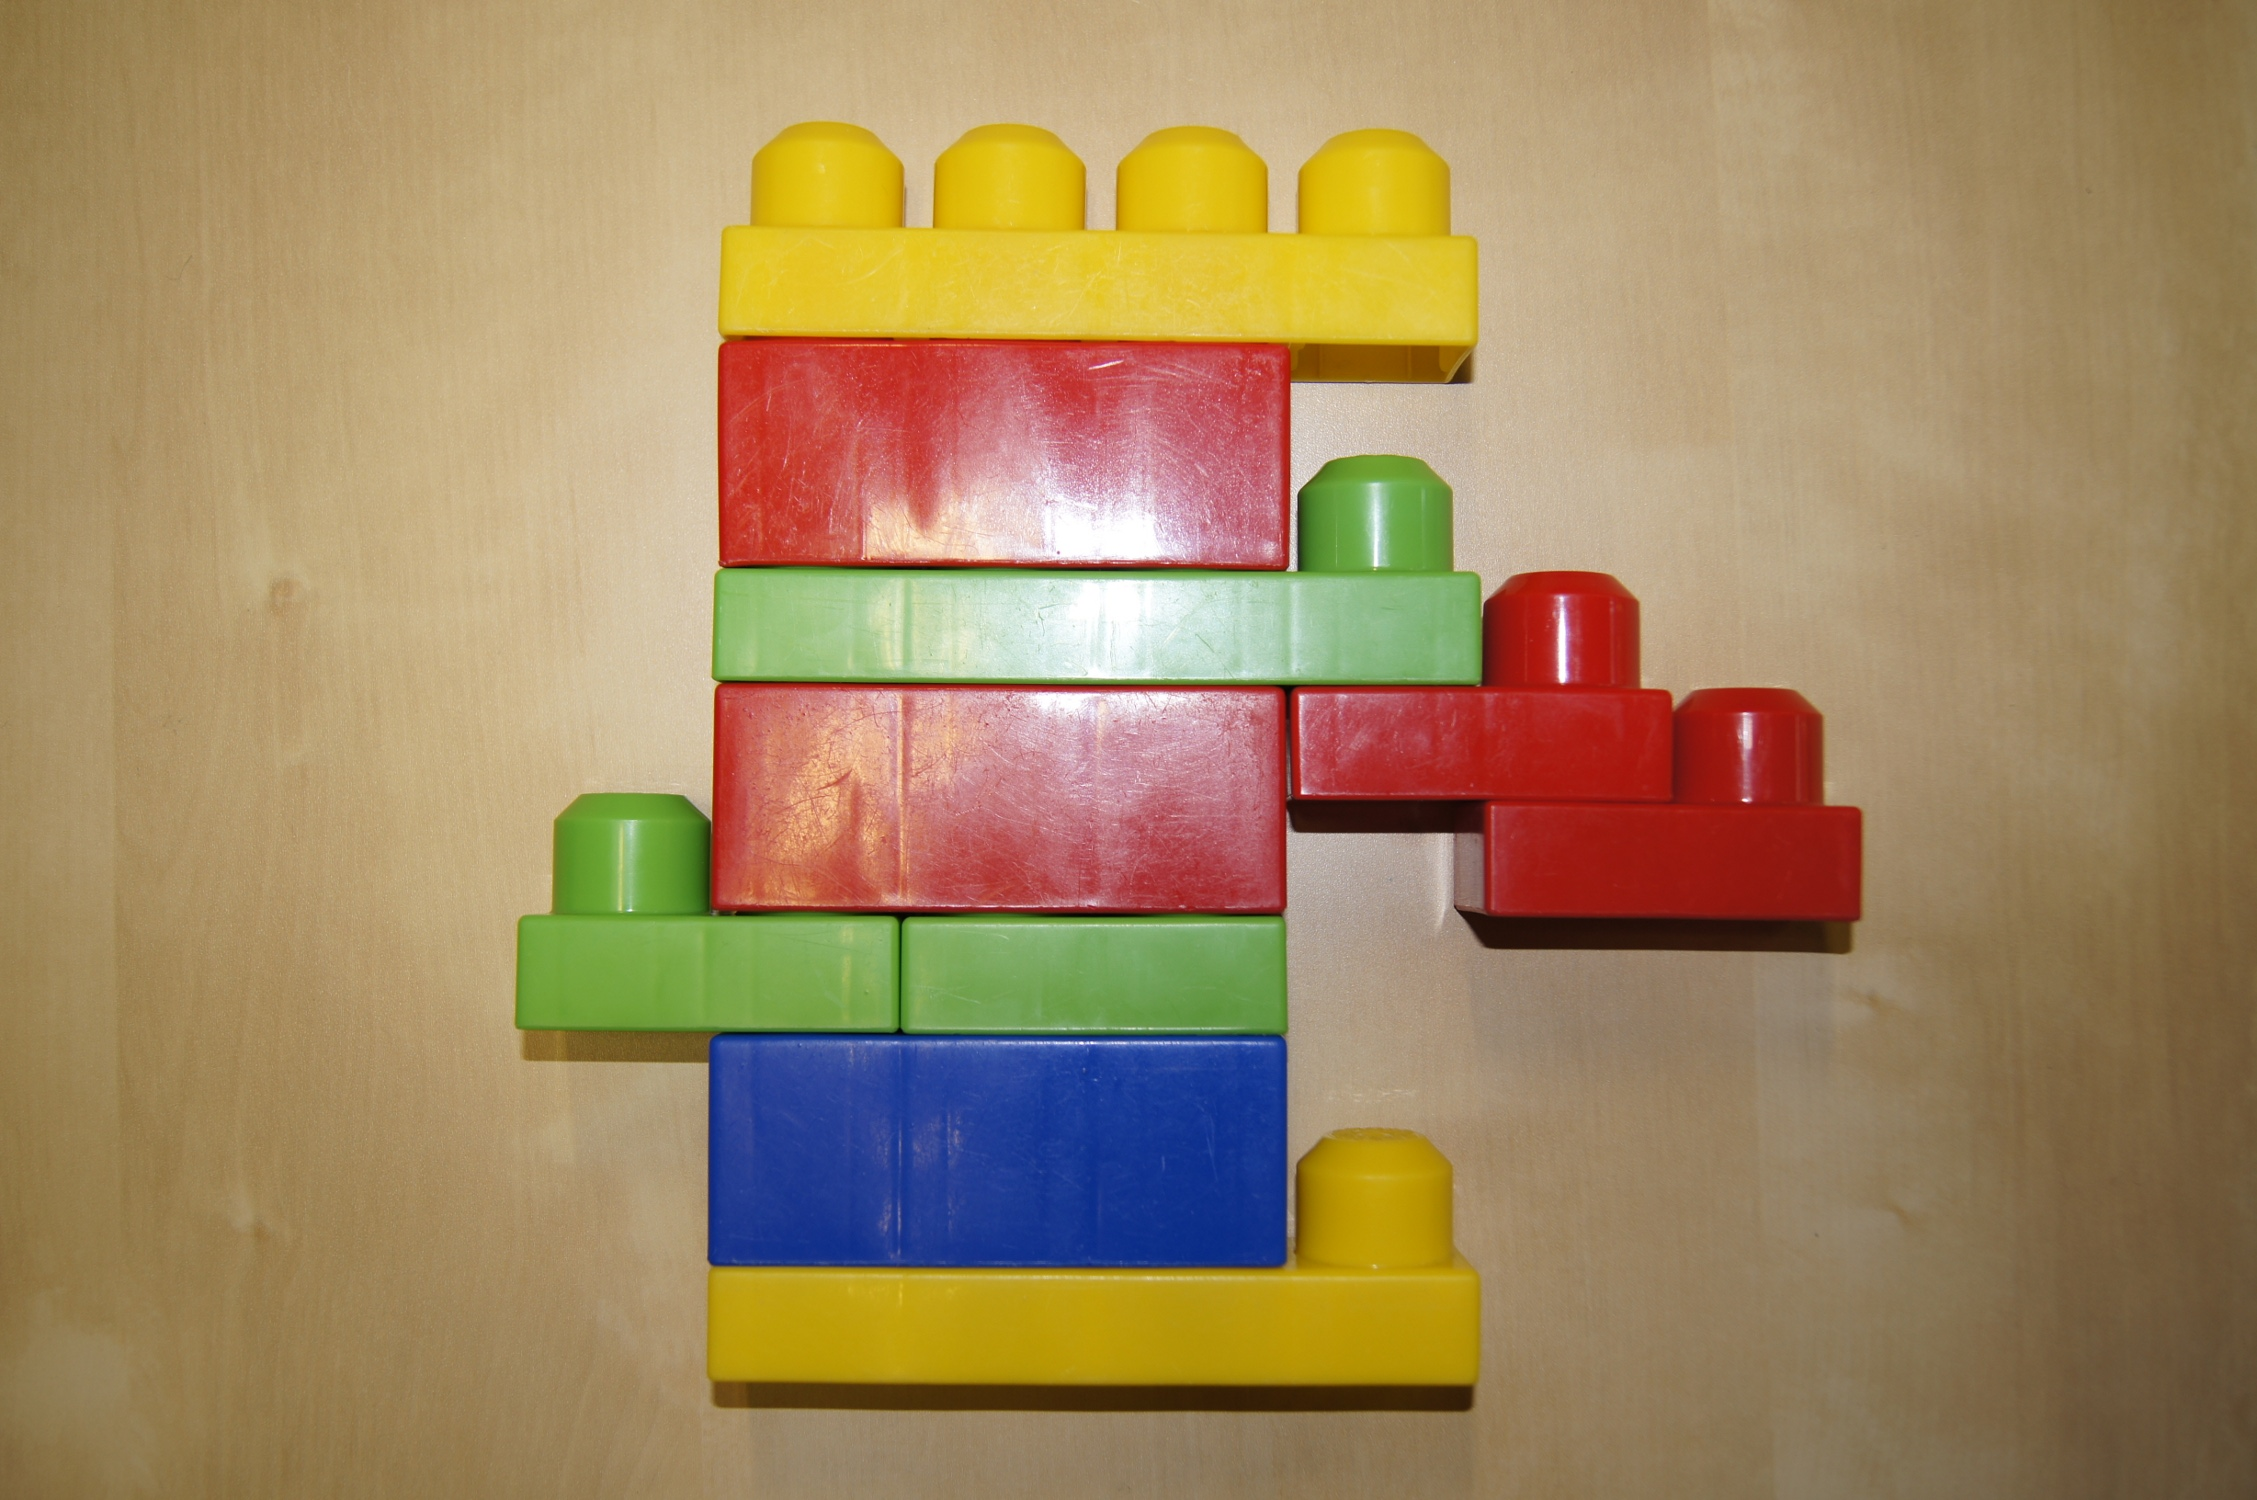
\includegraphics[width=0.24\columnwidth]{foo/_DSC4118.JPG}
		\caption{Four examples of construction presented to the teacher}\label{fig:constructions}
    \end{subfigure}
    \caption{}\label{fig:setup}
\end{figure}

\subsubsection{Procedure}

The study was conducted in two separate rooms. Teacher and learner never talked about the experiment before and were explained the task only once isolated in their respective rooms. After explaining the task to each participant, the experiment starts. We reduced as much as possible the pause between explanation and experiment's start, so as they could not try to elaborate a teaching/learning strategy before starting. 

The teacher saw the building area from the student side. The student saw symbols displaying on a screen as an indication of button pressed by the teacher. The learner manipulate the blocks and try to build the construction the teacher has in mind. The teacher presses the button so as to guide the student in building the construction it has in mind. A construction is made of any number of blocks at least linked by one pad. The manipulation of the button is the only way for the teacher to communicate with the learner. The spacial organization of button is different than the spacial organization of displayed symbol on the learner side. The teacher is aware that the mapping is different but not of the actual mapping. This way the teacher can not give direct spatial indication. The observation of the screen was the only way for the student to receive instructions from the teacher. The experiment stopped when the student decided the construction he had build was correct.

\subsection{Results}

For the experiment we did this summer, we recorded only the timing in button presses and the video the teacher was seeing. In addition, we took notes on both side (teacher/learner) on what participants where thinking, what buttons or displayed symbols meant, and the rough evolution of such meaning (not timed). We ran a total of 18 experiments, 14 were successful and 4 failed. The average duration of one experiment was 18 minutes with a minimum of 7 minutes and a maximum of 45 minutes.

The first analysis concerns types of instructions. When analysing the different types of instructions the participants were using, we created 9 categories.
\begin{enumerate}
    \item \textbf{Positive Feedback}
    \item \textbf{Negative Feedback}
    \item \textbf{End:} A signal identifying that the construction is finished 
    \item \textbf{Reset}
    \item \textbf{Guidance:} A signal informing what to do. It includes \emph{change, invert, revert, new block, continue, stack} 
    \item \textbf{Colour:} A signal referring to colour of a block. It includes \emph{yellow, blue, red, green}
    \item \textbf{Size:} A signal referring to size of a block. It includes \emph{small, medium, big}
    \item \textbf{Location:} A signal referring to location of a block. It includes \emph{under, above, left, right}
    \item \textbf{Group:} A signal referring to group of block. It includes \emph{in, out, group\_X}
\end{enumerate}

For each experiment, we then identified if the teacher or the learner consider each type of instruction. The results are shown in figure~\ref{fig:types_of_feedback}. We note that for every experiment the positive and negative feedback instruction were considered. In addition, the \emph{End} instructions is often considered while more concrete instruction such as \emph{Guidance, Colour, Size, or Location} were not much considered, especially by the student.

\begin{figure}[H]
	\begin{center}
   		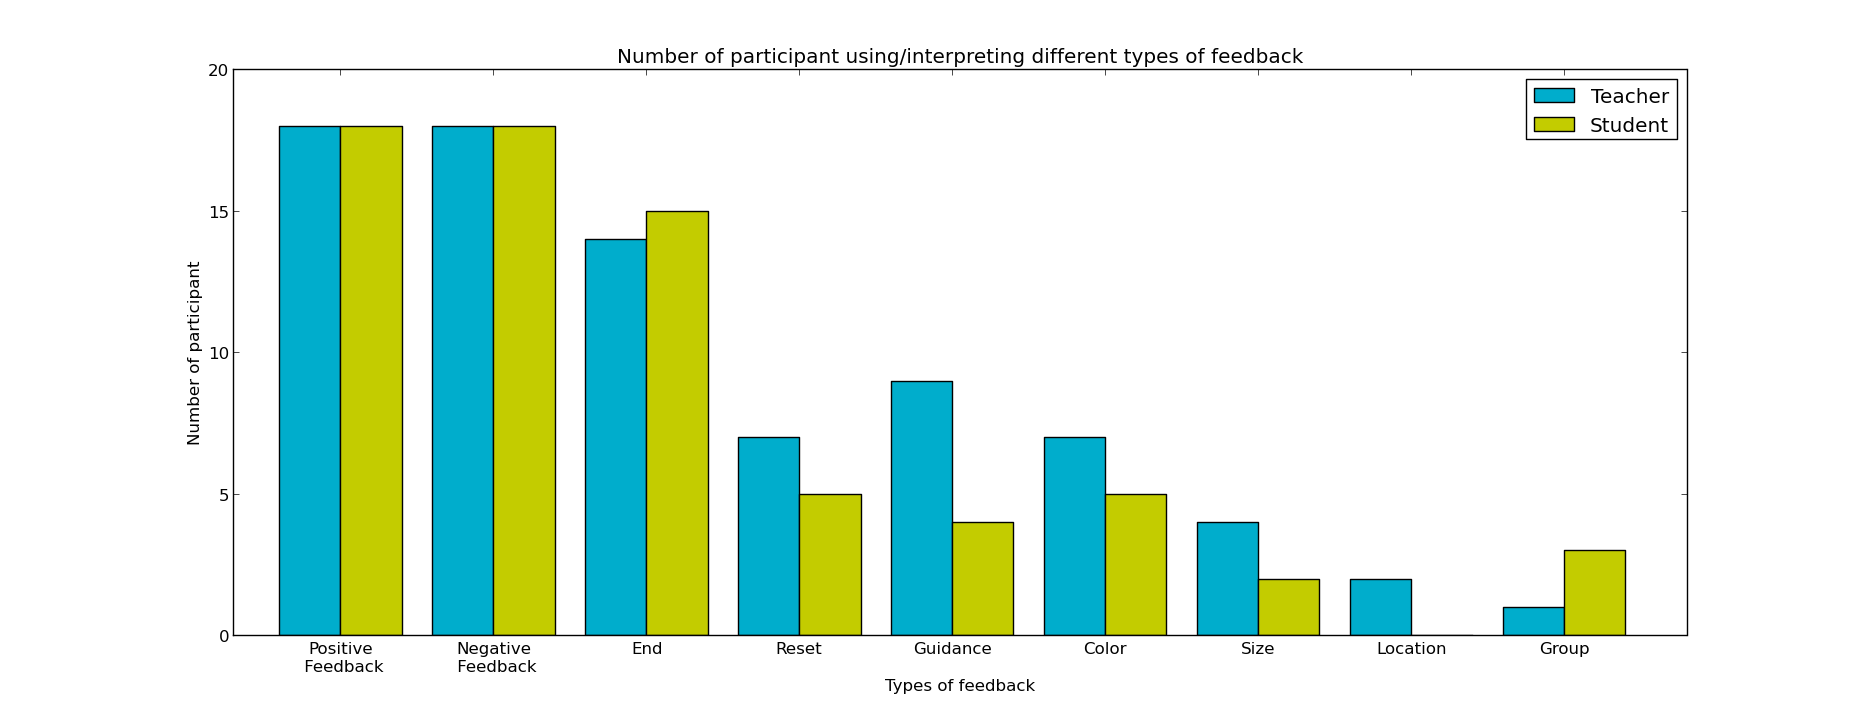
\includegraphics[width=\columnwidth]{types_of_feedback.png}
   		\caption{Number of participants that used (teacher) or interpreted (student) channels as conveying different types of instructions. All participants considered positive and negative feedback types of instruction.}
    \label{fig:types_of_feedback}
   	\end{center}
\end{figure}

From this results, it would be interesting to know to which extend the teacher and the learner understand each others. To do so, we compare the associated meaning of each button (or specific button pattern, e.g.\ all buttons pressed at the same time) at the end of the experiment for both teacher and learner. We can then count the number of button understood, misinterpreted, or ignored by the student. We can then average the results for successful and failed experiments, see figure~\ref{fig:types_of_understanding}.
We can note that for successful experiments, the average number of signal understood is 3.5 which mostly correspond to positive feedback, negative feedback, end, and occasionally reset when needed. Interestingly for failed experiments, this number drops to 1.2, with a larger amount of signals misinterpreted and ignored.

\begin{figure}[H]
	\begin{center}
   		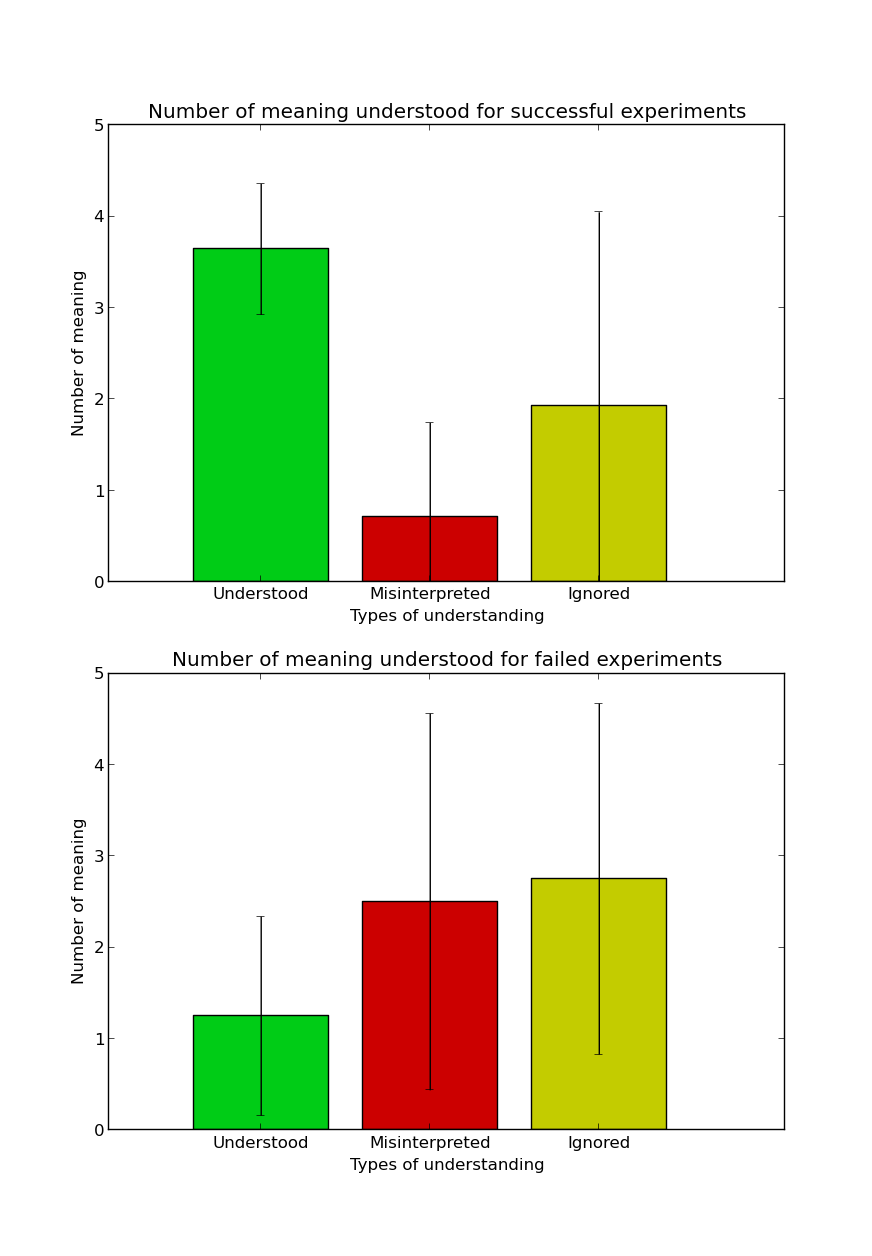
\includegraphics[width=0.4\columnwidth, trim=0cm 16cm 0cm 1.85cm, clip=true]{types_of_understanding.png}
   		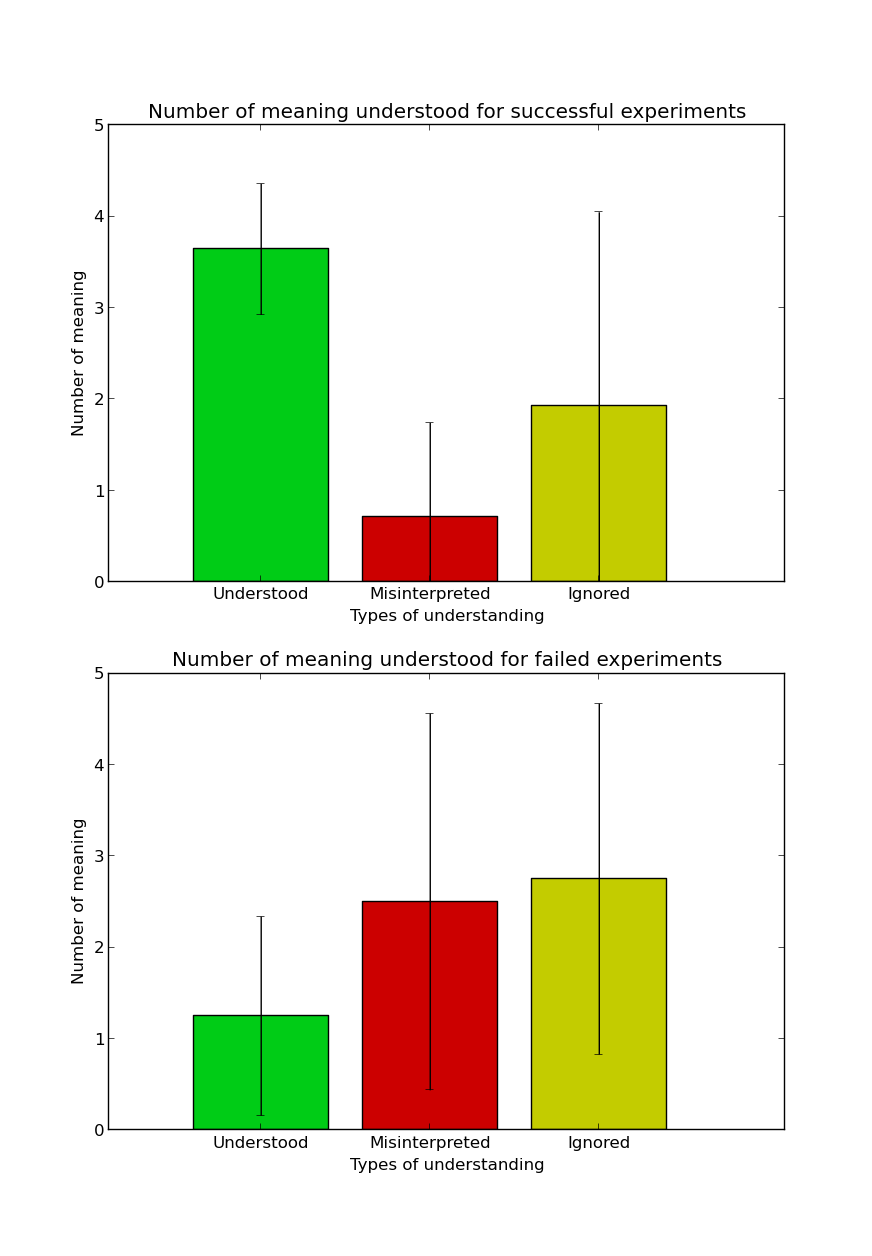
\includegraphics[width=0.4\columnwidth, trim=0cm 1.85cm 0cm 16.5cm, clip=true]{types_of_understanding.png}
   		\caption{Distribution of instruction channels that were understood, misinterpreted, and ignored by the learners. Data average across all learners for successful (left) and failed (right) experiments.}
    \label{fig:types_of_understanding}
   	\end{center}
\end{figure}

During the experiment, we noticed interesting properties on the feedback channels: some participants were inverting the meaning of such channel before, most of the time, detecting this misunderstanding and switching the meaning of button from positive to negative or the reverse. In few cases, it was the teacher that realized the learner were misinterpreting the signals but in most cases it was the learner that had to reinterpret the signals, often after a \emph{reset} instruction from the teacher. The data we collected are not enough detailed for this fine analysis but we are able to count the number of feedback interpretation switch per experiment, not their reason. This is shown in figure~\ref{fig:feedback_switch_enhanced}.

\begin{figure}[H]
	\begin{center}
   		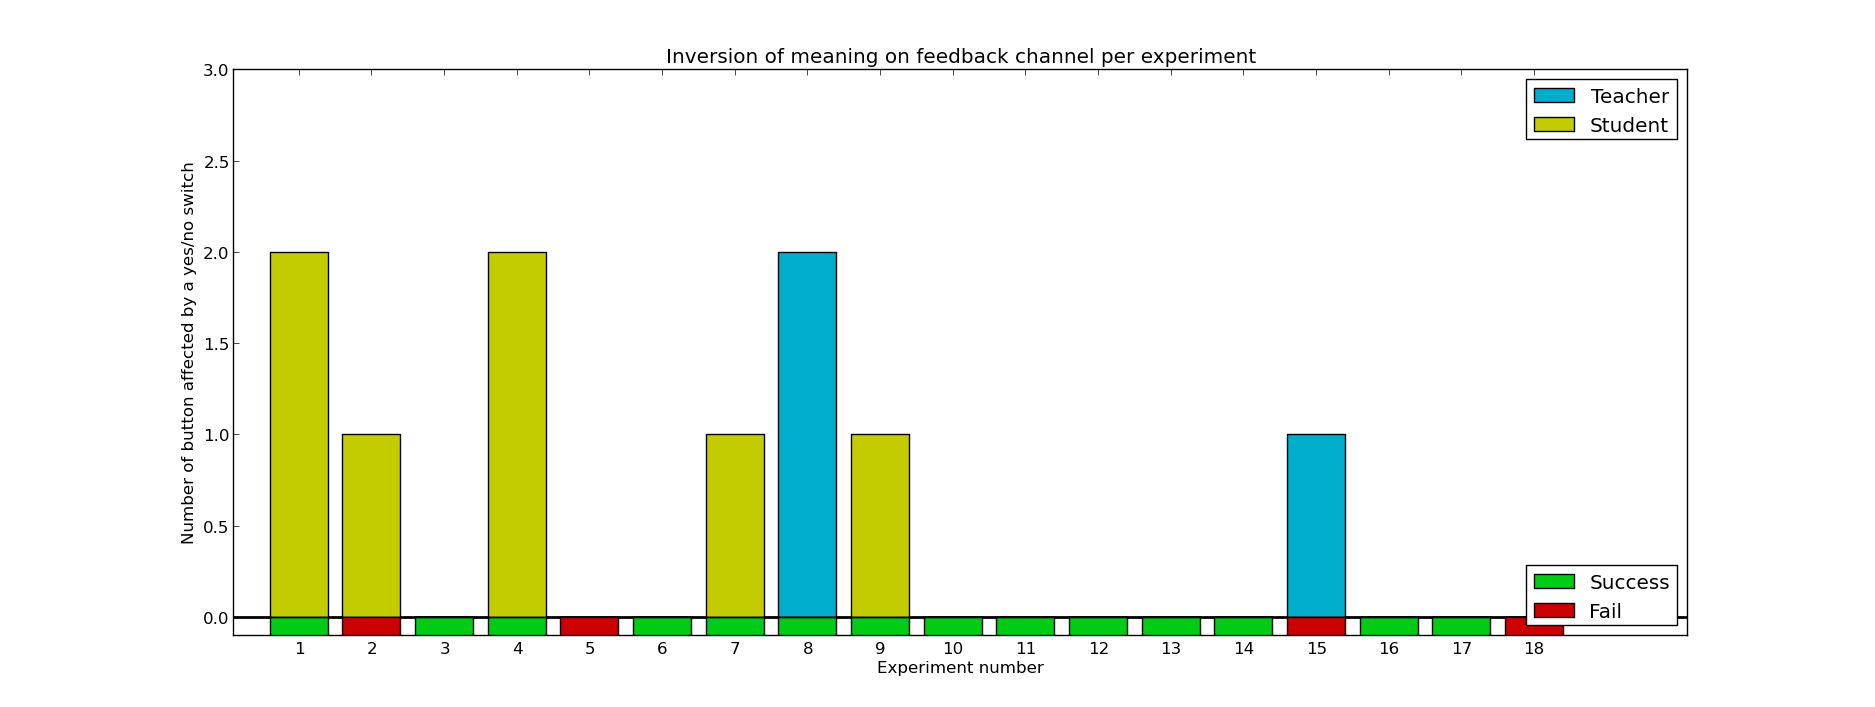
\includegraphics[width=\columnwidth]{feedback_switch_enhanced.png}
   		\caption{Number of channel whose meaning switch between positive and negative feedback during the experiment for the teacher and the student. In blue, cases when the teacher decides to change the meaning of a button from one feedback to the other. In yellow, cases when the student changed its interpretation of one button.The bottom coloured bar indicates if the experiment was successful or not. In 5 out of 14 successful experiments the teachers or the learners changed their use/interpretation of button between positive and negative feedback. A value of two indicate that student inverted the meaning of feedback channel, i.e.\ believing positive was negative and reversely, before either the teacher or the student fixed the misunderstanding.}
    \label{fig:feedback_switch_enhanced}
   	\end{center}
\end{figure}

An other interesting property is the context dependant meaning of some specific button presses patterns. For example, in several cases the teacher was pressing all buttons to signify a salient event. This event was either perceive as a \emph{Reset} instruction if the student felt lost or a \emph{End} instruction is the student felt confident about it understanding of the previous interaction sequences. This is illustrated in figure~\ref{fig:timeline}, where at $t=200 s$ the teacher presses all button to signify a \emph{Reset}. Indeed it seems he already tried several techniques with no success. After this \emph{Reset}, it starts again a new teaching techniques, which seems to work fine as the interaction keep going on the same track. Finally, to signify the end, the teacher send again the all buttons event which now means the task is completed. This signal is well understood by the student and the experiment goes to a successful end.

\begin{figure}[H]
	\begin{center}
   		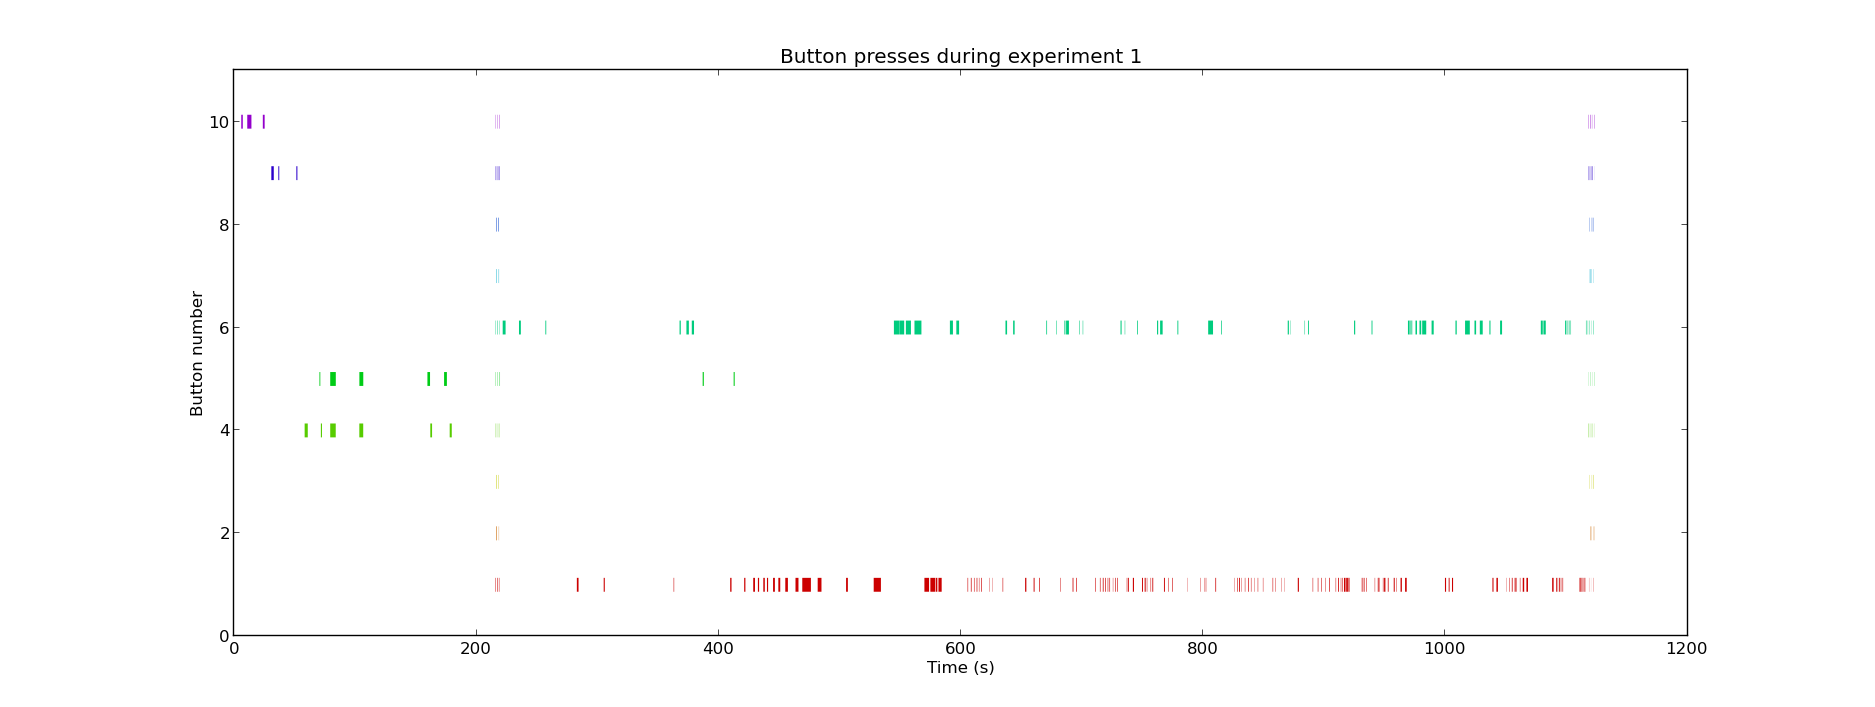
\includegraphics[width=\columnwidth]{timeline_experiment_1.png}
   		\caption{One full sequence of interaction, the events represent button press thought time and per channel. In this experiment the teacher, after trying several button, decided to send a ``reset'' signal by pressing all buttons. Then they successfully converged to a feedback based communication and are completing the task. At the end, the teacher signals the task is over by, once again, pressing all buttons.}
    \label{fig:timeline}
   	\end{center}
\end{figure}

Finally, figure~\ref{fig:understanding_per_feedback} is an attempt to describe what types of instruction where actually understood, misinterpreted, or ignored. While I still have to think and confirm the validity of this plot, it seems a good indication that positive and negative feedback, end, and reset are the most commonly understood instructions. 

\begin{figure}[H]
	\begin{center}
   		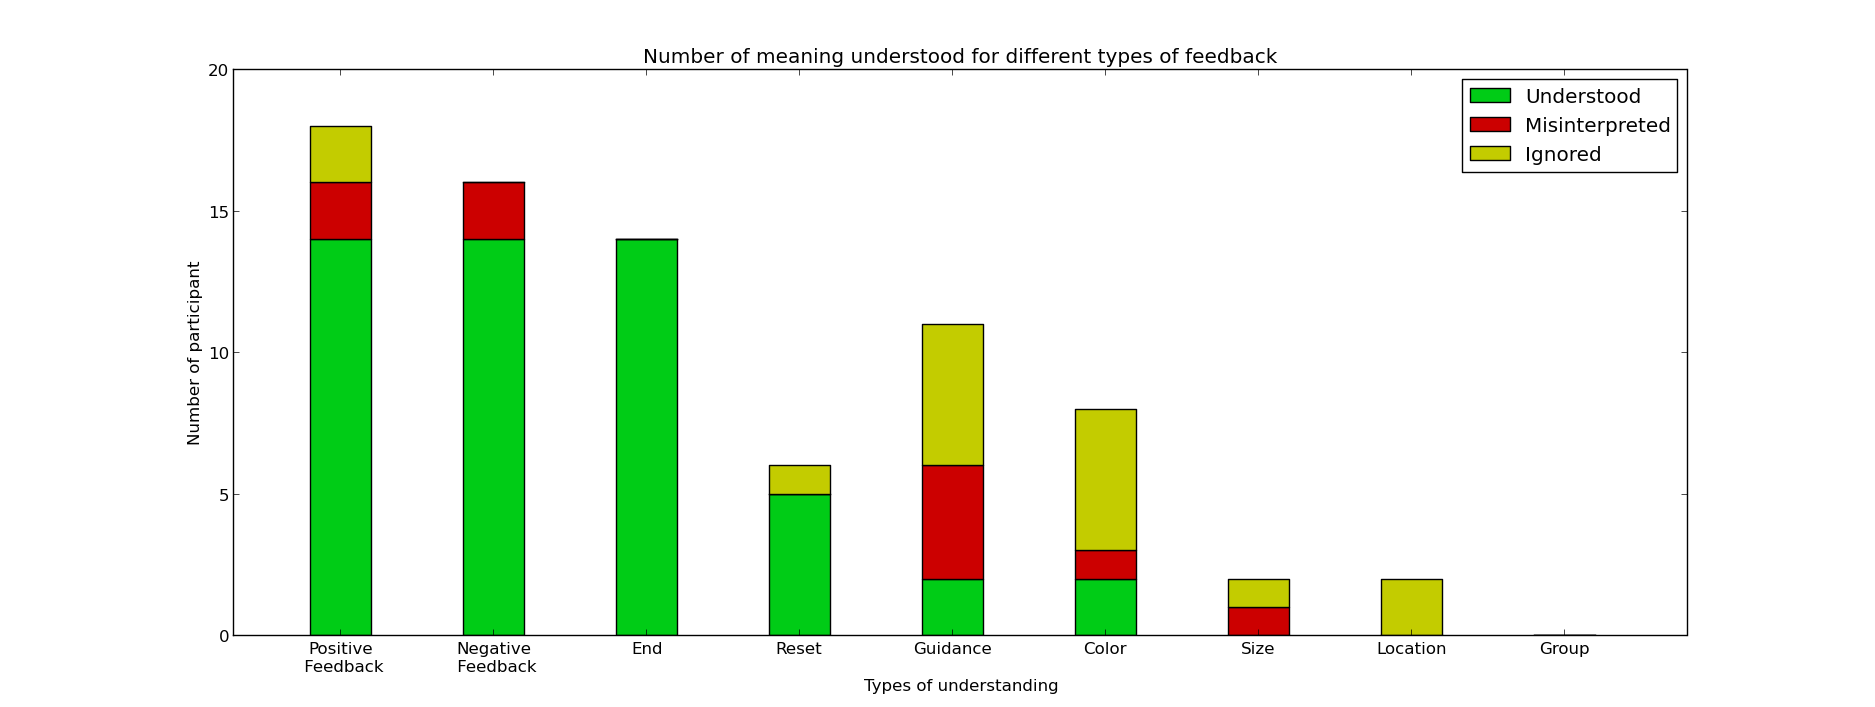
\includegraphics[width=\columnwidth]{understanding_per_feedback.png}
   		\caption{Learner type of understanding of different types of instruction from the teacher at the end of the experiment.}
    \label{fig:understanding_per_feedback}
   	\end{center}
\end{figure}

As a concluding remarks, I have also experienced some students affected by the so called confirmation bias. While interpreting negative feedback into positive they were going quite far in a wrong direction even if signal would seem contradictory for an outside observer. It was very difficult to re-assess their belief, they better thought the teacher was mistaking or were pursuing in a very improbable direction. I think no students were able to overcome the confirmation bias problem by themselves, leading either to a failed experiment or needed the teacher to produce a salient event to reset the experiment. With the recorded data, it is unfortunately not possible to quantify this phenomenon even if the figure~\ref{fig:feedback_switch_enhanced} gives a good first intuition.

\section{Comments on experimental design}

\begin{itemize}
    \item We can see the hand of the student, which may convey social cues.
    \item The information I decided to record is not enough for a proper analysis, we would need to record the full experiment on both side (user + objects) with participant speaking aloud. Ideally, we want to track, through time, the evolution of belief on both side. The more the time tracking is accurate the more we can count event for each meaning and their evolution.
    \item The colour of the button may be a bias for the teacher. But in an other perspective it helps to remember which button means what. Also, I heard that $7\pm2$ is in average the number of memory association untrained human can store (short/middle term). Then perhaps $10$ buttons is too much. Or more importantly, perhaps the only facts that this experiment is short terms bias it towards the use of simple, easy to remember, instructions.
    \item The construction the teacher asked the student to build may have some specific pattern and properties (symmetry, colour ordering, etc.) that may influence the learning. But those are common assumptions even when learning from known signals.
    \item From my personal experience, there is a little lag between both side (no more than 2 seconds). Streaming the video is not done the best way. It is transparent for the users, the only effect I can think of is that it slows down the interaction and may influence the user towards strong turn taking behaviours. May be good to fix.
    \item In recordings, have an explicit marker to known when experiment start and stop. 
    \item Would be better if we can extract high level information from the current construction without using laborious annotation process or automated image analysis. It may be good to implement the task on a computer, where the learner is using the mouse to build something on the screen. This way we can control what the teacher sees, what the learner can do, and what is the current state of the construction in a usable format.
    \item Would be good to have a measure of progress in the task. How much the task is completed, or how far the learner is going in a good of bad direction. It would enable to correlate signal understanding and task progression, to link reset event to negative performance, and to ``explain'' context relative meanings. If previous point implemented, this may be quite easy. 
    \item What is more relevant: press/release button events or the duration a button is hold pressed? This depends on the situation and is hard to analyse ``automatically''.
    \item How to analyse pattern in the use of one button, e.g.\ one press to mean ``no'', two press to mean ``yes''?
    \item The student reported difficulty to remember the symbols that were used before, perhaps queuing the last five symbols would help. 
    \item Student tends to use the following heuristic: ``the symbol I will receive the most will be a negative feedback''. If the teacher intend to provide it, it is a very good heuristic due to the construction task. Can we think of an other setup where it is no more a good strategy?
\end{itemize}


\bibliographystyle{ieeetr}
\bibliography{ref}

\glsaddall
\printglossary
\end{document}
